

\begin{frame}
        \frametitle{Method}
        \begin{block}{Because Cyclus is Agent-Based}
                \begin{itemize}
                        \item Its regions and institutions have the agency to dynamically make and alter deployment decisions.
                        \item Each agent can make their own predictions of the future based on current and past performance of the simulation.
                \end{itemize}

                We embedded advanced time series prediction algorithms to automatically
                deploy fuel cycle facilities for the user. This was implemented
                in \textbf{\texttt{d3ploy}}, an Institution agent.
        \end{block}
\end{frame}

%\begin{frame}
%  \frametitle{Goal of the Project}
%  % a comment
%  \begin{itemize}
%    \item[$\bullet$] Three types of methods were looked at for doing the prediction.
%    \item[$\bullet$] Non-optimizing methods. These methods included moving average
%                     , autoregressive moving average (ARMA), and autoregressive
%                     heteroskidasticity (ARCH) models.
%    \item[$\bullet$] Deterministic models. These models use a methodology that will
%                     always return the same answer given a unique input. This includes
%                     Fast Fourier Transforms, Exponential Smoothing, Holt-Winters,
%                     Polynomial regression.
%    \item[$\bullet$] Stochastic models. With stochastic models, the output is based
%                     on randomly sampling models to determine the behavior of the
%                     next time step. The method implimented here is a machine learning
%                     seasonal method.
%   \end{itemize}
%\end{frame}
%

  \begin{frame}
    \frametitle{Motivation}

    \textbf{Gap in capability: User must define when support facilities are deployed}

    \begin{figure}[htbp!]
      \begin{center}
        
\includegraphics[width=0.8\textwidth]{images/user-deploy}
      \end{center}
            \caption{User defined Deployment Scheme }
    \end{figure}

    \textbf{Bridging the gap: Developed demand-driven deployment capability in \Cyclus. This capability is named \deploy.}

    \begin{figure}[htbp!]
      \begin{center}
        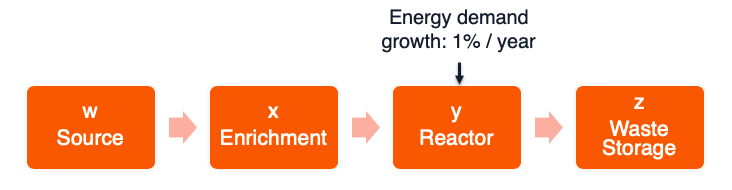
\includegraphics[width=0.8\textwidth]{images/auto-deploy}
      \end{center}
            \caption{Demand Driven Deployment Scheme}
    \end{figure}

  \end{frame}
